\documentclass[article]{aaltoseries}
\usepackage[utf8]{inputenc}
\usepackage{hyperref}
\makeatletter
\g@addto@macro{\UrlBreaks}{\UrlOrds}
\makeatother
\usepackage{amssymb,amsmath}

\begin{document}
 
%=========================================================

\title{Technical and Financial Evaluation of Managed Kubernetes Service Providers in Seasonal Student Radio Context}

\author{Aarni Halinen
\\\textnormal{\texttt{aarni.halinen@aalto.fi}}}

\affiliation{\textbf{Tutor}: Mario di Francesco}

\maketitle

%==========================================================

\begin{abstract}

Radiodiodi is a seasonal non-profit student-driven radio station which manages all technological aspects of a radio station. Over the years the infrastructure has grown hard to understand  and  maintain, and to combat this, Radiodiodi is  moving towards a cloud-native approach with Docker and Kubernetes. This paper studies and compares feature and business aspects between three major service providers Amazon Web Services, Google Cloud and Microsoft Azure. The evaluation is conducted by comparing documentation as well as deploying a Kubernetes application to every evaluated platform.

\vspace{3mm}
\noindent KEYWORDS: Cloud-native, Docker, Kubernetes, PaaS, Amazon Web Services, Google Cloud, Microsoft Azure

\end{abstract}

\newpage

%============================================================


\section{Introduction}

Radiodiodi is a  non-profit seasonal student-driven radio station founded in 2012 at Aalto University. Radiodiodi organizes a two-week radio broadcast every year in April from a mobile studio built on the campus. The recorded program is digitally processed on-premise and broadcast over FM and the internet.

Radiodiodi manages all technological aspects of a radio station.  Over the years, the infrastructure and the overall setup has grown hard to understand and maintain. The current infrastructure consists of a number of non-standardized server machines and operating systems in complicated networking setups. Furthermore, there has been no standard way of deploying the services on the server machines.

To combat the issues of complicated networking setups and non-standardized servers and service deployment, Radiodiodi is moving towards a cloud-native approach. Cloud-native computing is an approach to building and running scalable applications in modern cloud environments \cite{cncf}. Common characteristics of cloud-native are for example  microservice architecture and the use of containers. Docker container runtime and Kubernetes container orchestration are examples of common cloud-native technologies.

In fall 2019, a prototype Kubernetes setup was deployed on a lightweight K3s distribution installed on virtual machine server purchased from Digital Ocean \cite{tuomihalinen2019}. However, the prototype setup has no guarantees for being production-ready. The setup runs on a single, low performance virtual machine which runs both Kubernetes control plane and all the services. The deployment is most likely not capable of handling high load scenarios such as broadcasting season. Furthermore, adding extra computing power to the deployment is more complicated compared to managed Kubernetes services. Moreover, no performance or business aspects like pricing have been evaluated for the setup.

This paper studies whether different cloud services offer better capabilities for Radiodiodi. The evaluation focuses on pricing and features of managed Kubernetes and storage services. Cloud service providers evaluated in this reports are Amazon Web Services, Google Cloud Platform and Microsoft Azure. Evaluation is conducted by comparing documentation as well as deploying the cloud application to every evaluated platform.

\newpage
\section{Cloud-native computing}

\subsection{Definition}

Cloud-native computing is an approach to building applications that are designed to be running in a cloud. The cloud-native approach enables loosely coupled, scalable, resilient, manageable and observable systems to be built and run in dynamic cloud environments \cite{cncf}. The approach is exemplified by technologies such as containers, microservices, immutable infrastructure and declarative APIs.

Kratzke and Nint \cite{kratzke2017understanding} define cloud-native application as \textit{a distributed, elastic and horizontally scalable system composed of (micro)services which isolates state in a minimum of stateful components. The application and each self-contained deployment unit of that application is designed according to cloud-focused design patterns and operated on a self-service elastic platform.} The definition itself is not self-explanatory, and requires understanding of further terminology.

\textbf{Elasticity} refers to the degree to which a system is able to automatically adapt to workload changes \cite{herbst2013elasticity}. The system provisions and de-provisions resources such that the current demand is always matched as closely a possible. When application costs are relative to resource usage, elastic services tend to keep costs at minimum without sacrificing performance.

\textbf{Structural scalability} refers to the ability of a system to expand horizontally or vertically without major modifications to its architecture \cite{bondi2000characteristics}. Vertical scaling means scaling by adding power, while horizontal scaling means scaling by the amount of machines. Scalability also takes into account the system's ability to function without undue delay or unproductive resource consumption at different levels of load \cite{bondi2000characteristics}. This is called load scalability.

\textbf{Microservices} are, in contrast to monolithic services, an architectural style of building application as a suite of multiple small services \cite{fowler2014microservices}. Each service is running in its own process and the application's data flow is achieved with lightweight communication between the services.

For example a simple web-based file-upload application could consist of a REST API service for accepting user's files, which in turn communicates with different process actually responsible for storing and processing the file. The communication between services could be handled with HTTP.

\textbf{Self-contained deployment unit} is \textit{a part of the application’s deployment topology for realizing a specific technical unit} \cite{inzinger2014madcat}. The deployment unit is nowadays often understood as a container. Most popular of the container technologies is Docker, which will be discussed more detailed in the section \textbf{\ref{2.2}}.

\textbf{Stateful components} refer to parts of application that have state, such as databases. Stateful components are used to synchronize internal state to provide a unified behavior for a scaled-out application \cite{fehling2014cloud}.

State is important in cloud-native applications since it interferes with horizontal scaling; for example the application's responds might become non-deterministic if databases are scaled horizontally and state is split between instances.

\subsection{Docker}
\label{2.2}

Docker is a containerization platform for developing, deploying and running applications \cite{docker}. Docker attempts to erase issues that arise from running the application in different infrastructures and environments, such as different operating systems (OS) and compilers, by packaging the application environment within the application container.

\begin{figure}[hbt!]
    \centering
    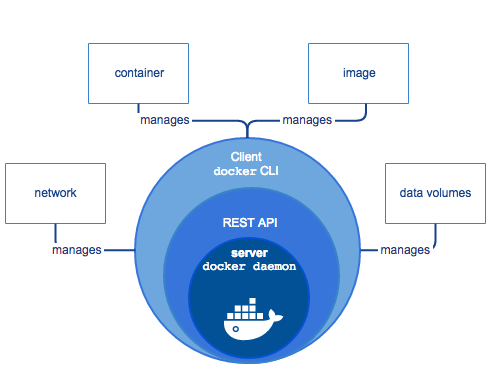
\includegraphics[width=140mm]{figures/docker-engine.png}
    \caption{Components of Docker engine \cite{docker}.}
    \label{fig:docker-engine}
\end{figure}
\newpage

The Docker engine consists of three major components: Docker daemon, Docker REST API and Docker client \cite{docker}. The components are illustrated in Figure \ref{fig:docker-engine}. The daemon manages and creates the docker objects, and the REST API is the interface for applications to communicate with the daemon. Docker client is a command-line interface (CLI) which utilizes the REST API for communication.

The basic types of Docker objects are containers, images, volumes and networks \cite{docker}. Docker containers are runnable instances which are defined by read-only templates called images. Images contain the configuration details about the application and its environment. The images are often based on another images, for example a operating system image, with some additional configuration. Applications that require persistent data storage use volumes. Volumes are managed by the Docker daemon instead of the host file system. Docker networks are used to connect multiple containers together.

Started as a open-source project in early 2013, Docker has become de-facto containerization platform in the industry. The Docker images are lightweight in comparison to virtual machines, since they do not require a virtualization hypervisor to run \cite{docker}. Docker containers operate on top of already running host operating system and utilize host's kernel directly \cite{merkel2014docker}. This has two significant benefits. First, an idle container is not using computing resources. Second, the starting and stopping of container is similar to starting and stopping an application, and there is no need to boot and shut down a whole OS.

\subsection{Kubernetes}

Kubernetes (K8s) is a container orchestrator, i.e. a platform for managing containerized workloads and services \cite{k8s}. Developed by Google, it was open-sourced in 2014 and has since then
grown to be the product of choice for building cloud-native applications \cite{hightower2017kubernetes}. In 2020 it is present in nearly every public cloud.

Kubernetes provides a framework for running containerized applications resiliently in a distributed system \cite{k8s}. Kubernetes provides horizontal scaling, automatic rollouts and rollbacks when updating containers, restarts, replaces and kills failing containers and allows for storing and managing application secrets.

Most often an application of microservices is described to Kubernetes in a declarative manner using \textit{declarative object configuration} \cite{k8s-obj-man}. The configuration tells Kubernetes the desired state of the cluster \cite{hightower2017kubernetes}. Using this information, Kubernetes automatically tries to create that state \cite{k8s-objects}. The configuration specifically describes what containers are running, what resources are available for the containers and what policies, such as restart, upgrade and fault-tolerance, are configured for the containers.

The declarative nature of Kubernetes makes it easy to implement scalability and elasticity. Adding a new replica of a service is one-line change into the configuration describing the desired state. The Kubernetes ensures that the new replica is actually being run. Scaling is also achieved by deploying new nodes to the cluster. Kubernetes automatically handles the deploying of pods to the new nodes.

Kubernetes also supports imperative object management \cite{k8s-obj-man}. Imperative commands operate on live objects and it is recommended only for development use. Imperative object configuration operates on an individual file. However, it does not support multiple writers since updates to live objects must be reflected in the configuration. Updates missing from declarative configuration will be lost on next replacement.

\begin{figure}[hbt!]
    \centering
    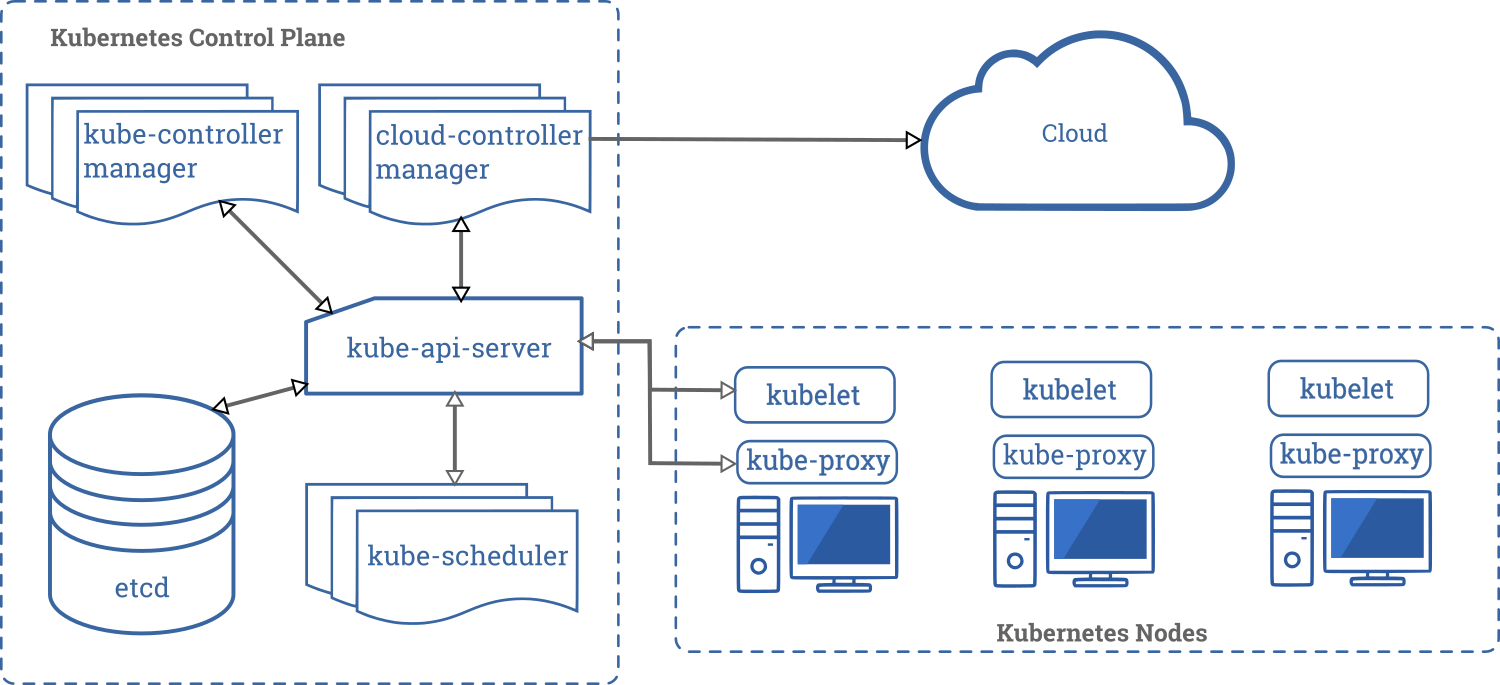
\includegraphics[width=150mm]{figures/k8s.png}
    \caption{Diagram of a Kubernetes cluster with all the components tied together \cite{k8s-comps}.}
    \label{fig:k8s-figure}
\end{figure}

Kubernetes API is used to send configuration objects to Kubernetes. The user may use the API directly, but most often a CLI tool called \textit{kubectl} is used to make the API calls \cite{k8s-objects}. Most often, the information is provided to \textit{kubectl} in a \texttt{.yaml} file which is automatically converted to JSON when the tool calls the API. The API gives instructions to Kubernetes' orchestration layer called control plane, which makes sure that the actual state of every object matches the desired state of the application.

In Kubernetes, application is deployed into a cluster. Clusters consists of at least one worker machine called node \cite{k8s-comps}. The worker nodes host the pods, which are the basic execution unit of a Kubernetes application \cite{k8s-pods}. A Pod is a representation of processes running in a cluster. It encapsulates the application's container, storage resources, IP addresses as well as controls how the container should run.

Usually, a single container is run within a single pod, but pods also support multiple containers for tightly coupled services \cite{k8s-pods}. Containers in a pod are located and scheduled on the same machine in the cluster. Each container has a unique IP address, and containers inside a pod can communicate on the \textit{localhost} interface. Similar to Docker, pods can specify persistent storage called volumes. All containers within the pod can access the volume.

\subsection{Cloud service providers}

Traditionally, cloud computing services are divided into three levels of service offerings called \textit{Infrastructure as a Servic}e (IaaS), \textit{Platform as a Service} (PaaS) and \textit{Software as a Service} (SaaS) \cite{bhardwaj2010cloud}. IaaS is a form of cloud hosting, where the provider delivers the network access, routing services and storage. SaaS is a hosted set of software that the user does not own but pays for the utilization of its features.

PaaS is a type of service, in which the hardware plus a base layer of application software is provided for the user \cite{bhardwaj2010cloud}. It facilitates development and deployment of user's applications without the need to manage the underlying infrastructure or the software. Depending on the nature of the service, the base application software can be for example database or container runtime. Managed Kubernetes services are considered PaaS.

A number of cloud service providers have sprung up after the introduction of Amazon's Simple Storage Service (S3) in 2006. The biggest providers in 2017 were Amazon with Amazon Web Services (AWS), Microsoft with its Azure platform, Alibaba and Google Cloud Platform (GCP) \cite{gartner}. Each of the aforementioned providers have a managed Kubernetes service. In this paper, we are going to focus on the AWS, Azure and Google Cloud platforms and their Kubernetes services.


\newpage
\section{Approach and methods}
\label{Criterias}
This paper looks to find an answer to which of the previously mentioned managed Kubernetes services would be best suited for use in Radiodiodi. The services are evaluated from usability, pricing and feature perspectives. The configuration created in fall 2019 is deployed to each of the platforms for evaluation. Furthermore, each platforms documentation is used to evaluate pricing.

\subsection{Service requirements}

Most of Radiodiodi's services are on low usage when Radiodiodi is not broadcasting. The services should be scalable since most of the load is generated during the broadcasting period. The services that are only required during broadcasting should be scaled down or even stopped during off-season. Because of the seasonal nature of service load, the network load is left out of the scope of the evaluation.

In the existing Kubernetes configuration, the \textit{referenssi} container constantly records the broadcast and writes numerous Gigabytes of \texttt{.ogg} files for legal purposes. The service is operational only during the broadcasting period, and requires access to persistent storage during the broadcast.

\subsection{Pricing}

The most important evaluating criteria is the cost of running the existing Kubernetes configuration in each platform. The cost is evaluated by calculating the monthly price tag for running the configuration. The pricing data is checked from official documentation as well as from the platform specific billing page for each deployment. For evaluating the managed storage solution, a monthly price of transferring and storing 100 Gigibytes data is calculated for each of the platforms.

\subsection{Ease of deployment}

One of the main reasons for Radiodiodi to move towards a cloud-native approach is to simplify the management of the infrastructure. The prototype setup already covered the changes and configuration needed for the service code, which is therefore out of the scope of this paper.

The ease of deployment is evaluated by deploying the existing Kubernetes configuration to each managed Kubernetes service. The evaluation consists of changes needed to the configuration as well as installation of provider specific CLI tools. The extra configuration needed for turning on the key features is also evaluated.

\subsection{Features}

The most important features evaluated are existence of native resource monitoring, the ability to group nodes and automatic scaling of nodes. Since most of current services require low resources, the ability to group nodes into high and low performance nodes is preferred. Thus, the most resource-hungry services could be assigned to the more expensive nodes.

The key features being compared in this paper are:
\begin{itemize}
\item Automatic minor version updates
\item Kubernetes version upgrades Master and worker nodes together
\item Available Kubernetes versions
\item Resource monitoring built within the platform
\item Ability to deploy target pods at specific nodes (Node groups)
\item Closest availability zone
\item Auto-scaling
\end{itemize}

\newpage
\section{Results}

For easier comparison of costs, each Kubernetes deployment consisted of three worker nodes. Also, similar computing engines were selected for each deployment. EKS was deployed on \textit{t3.medium}, AKS on \textit{B2s} and GKE on \textit{n1-standard-1} instances. Each instance on EKS and AKS had 2 virtual CPUs and 4 GB of RAM. GKE's \textit{n1-standard-1} instances had 1 vCPU and 3.75 GB of memory each.

\subsection{Deployment}

Deployment of the existing Kubernetes configuration required only minor modifications to \texttt{.yaml} files. For saving the reference audio, the prototype had a \textit{sshfs} mount which could not be accessed without extra configuration. Many of the containers had a \textit{nodeAffinity} configuration, which was used to deploy the container onto a specific node. These lines of configuration had to be removed from the cloud deployment configuration. Furthermore, the load balancer \textit{caddy} had TLS configured, which had to be turned off since DNS records were not configured for the deployments.

After these changes, the configuration was deployable to any of the cloud providers. The clusters were created with cloud providers' web consoles, even though it was possible to use CLI for every provider. On the other hand, authentication and deployment were done with CLI tools.

The easiest deployment was for the GKE. Google Cloud uses Google authentication as authentication system, so Radiodiodi's GSuite authentication could be used. The cluster and a node pool of three \textit{n1-standard-1} instances were easy to create from the console, and the creation process itself included the selection of features such as automatic update (under the name of Release Channels) and node pool auto-scaling. After successful creation of the cluster and node pool, the \textit{gcloud} CLI tool was used to login into Google Cloud, after which the \textit{kubectl apply} operation was used to deploy the configuration. The deployment was successful and resources could be monitored within the Kubernetes Engine in Google Cloud.

The deployment to AKS was quite similar to GKE. The deployment required Microsoft account for authentication and installation of Azure CLI (\textit{az}) to get Kubernetes credentials for \textit{kubectl}. However, AKS does not list the cluster's services anywhere in the web portal. The easiest approach to finding \textit{caddy}'s IP address is to use \textit{kubectl get service}. Furthermore, container logs are hard to find within the portal. Compared to GKE, where the logs are found under \textit{Pod details} that is easiest accessed from \textit{Service details}, AKS hides container logs under \textit{View in analytics} button found on \textit{Insights} page.

EKS had the most difficult deployment. The deployment required creation of numerous roles with the \textit{AWS Identity and Access Management} tool. The cluster creation required extra attention, since Kubernetes can be deployed in two ways. EKS pods can be deployed on AWS Fargate \cite{fargate}, which is a proprietary server provisioner. Fargate eliminates the need to manage server nodes, but it does not support Kubernetes' Classic and Network load balancers \cite{ekslb}, like \textit{caddy} service in the used configuration. After configuring the cluster and node groups the deployment required updating local Kubernetes configuration with \textit{aws eks update-kubeconfig} and deploying the configuration with \textit{kubectl apply}.

\subsection{Costs}

The monthly price for running a Kubernetes cluster on any of the platforms consists of possible hourly maintenance fee for the cluster $m_{fee}$ and the prices for running the node computers. The price of nodes depends on the price on single node multiplied by the amount of nodes $p_{node} * N_{node}$. A VAT of 24 \% is added to each monthly billing.

Thus, monthly price is calculated as
\begin{equation}
    P_m = (m_{fee} * 24 * 31 + p_{node} * 3) * 1.24
\end{equation}

\subsubsection{Google Kubernetes Engine}

GKE has no maintenance fee for clusters. The price of single \textit{n1-standard-1} instance is \$26.73 per month \cite{gkeallpricing}. Google Cloud offers a 30\% discount for instances running over 730 hours a month, thus

\begin{equation}
\begin{split}
    P_m &= (0 * 24 * 31 + 26.73 * 3) * 0.7 * 1.24 = \$69.60
\end{split}
\end{equation}

However, the daily cost of the test deployment was \$4.80, excluding VAT, according to project's billing page. The monthly price with VAT based on the daily price would be \$184.51. This price does not contain the discount. According to cost table, the monthly price for used CPU cores and RAM were \$104.88. The rest of the price consisted of network load balancing forwarding rule and used server storage capacity.

Furthermore, on June 6, 2020, GKE will introduce a management fee for each cluster at \$0.10 per cluster per hour, except for one zonal cluster per billing account, which remains free of charge \cite{gkepricing}.

Google Cloud offers a managed NFS called Filestore, which can be configured as a Kubernetes persistent volume. However, the smallest provision is 1TB and costs \$200/month. The second option, which requires bit more configuration, is to use Compute Engines \cite{gkestorage}. The price for provisioned storage in this case is \$0.044 per GB per month \cite{gkestorageprice}, which implies monthly price tag of \$4.4.

\subsubsection{Azure Kubernetes Service}

AKS has no cluster maintenance fees. The cost for a single B2s instance is \$32.85 \cite{akspricing}.

\begin{equation}
\begin{split}
    P_m &= (0 * 24 * 31 + 32.85 * 3) * 1.24 = \$122.20
\end{split}
\end{equation}

Network, storage, load balancing and virtual machines had a daily cost of \$4.84. The monthly price according to deployment was \$150.04, excluding VAT and Azure monitor pricing. Even though resource monitoring is one of the evaluated features, it is left out of the equation because of the price. The log data ingestion to analytics tool costs (\$5.61) daily, which results in a total monthly price of \$323.95, excluding VAT, for the deployment.

Azure offers static and dynamic persistent volumes for Kubernetes \cite{aksstorage}. The price for storage in Azure files Standard plan is \$0.06 per used GB \cite{aksstorageprice}, excluding transaction costs, which means the 100GB storage would cost at least \$6.00 per month.

\subsubsection{Elastic Kubernetes Service}

EKS costs \$0.10 per hour for every cluster \cite{ekspricing}. Each \textit{t3.medium} node has a monthly price of \$31.54. Thus,

\begin{equation}
\begin{split}
    P_m &= (0.1 * 24 * 31 + 31.54 * 3) * 1.24 = \$209.58
\end{split}
\end{equation}

The test setup was run for 44 hours, and was priced at \$19.93, VAT included. A monthly price based on these 44 hours would be \$337.00.

Amazon Elastic File System (EFS) can be configured as a persistent volume for EKS deployments \cite{eksstorage}. EFS can be configured in
Standard mode which costs \$0.30 per GB per month, or in Infrequent Access mode. In Infrequent Access mode, the cost drops to \$0.025 per GB per month, but price for data transfer is \$0.01 per GB. Assuming the transferring of 100GB of recorded broadcast during one month, the price for 100 GB of storage is \$3.50.

\subsection{Feature comparison}

Some differences between features were noted during the deployment to each platform. The results are presented in the following table:

\begin{table}[hbt!]
\centering
\begin{tabular}{ |c|p{7em}|p{5.5em}|p{9em}| }
\hline
\multicolumn{4}{|c|}{Comparison results} \\
\hline
Evaluation criteria & EKS & AKS & GKE \\
\hline
Automatic updates
& No
& No
& 3 different release channels. \\
Master \& Node upgrade & Both manually & Yes & Yes \\
Kubernetes versions & 1.14, 1.15, 1.16 & 1.14, 1.15, 1.16, 1.17 & 1.14 , 1.15, 1.17 \\
Resource Monitoring & No & Costs extra & Yes \\
Node groups/pools & Yes & Yes & Yes  \\
Availability & Sweden & Ireland & Finland  \\
Auto-scaling & Yes & Yes & Yes  \\
\hline
Ease of deployment & 3rd & 2nd & 1st \\
Monthly price (docs) (\$) & 209.58 & 122.20 & 99.44\footnotemark \\
Monthly price (\$) & 337.00 & 186.05 & 184.51 \\
Storage price (\$) & 3.50 & 6.00 & 4.40 \\
\hline
\end{tabular}
\caption{Evaluation results \cite{eks}\cite{gke}\cite{aks}.}
\label{tab:template}
\end{table}
\footnotetext{Price without the 30\% discount for instances running over 730 hours a month.}

The most important features defined in section \textbf{\ref{Criterias}} are implemented by every platform, except for native resource monitoring in EKS. GKE is the overall best choice based on features. Currently, it is the only platform with automatic updates. Otherwise, the features are matched by AKS. It should also be noted, that GKE does not provide a Service Level Agreement (SLA) for Kubernetes version 1.17 and the Rapid release channel.

Based on the results, Google Cloud would be the best choice of the three platform to run Radiodiodi's cloud-native services. It has the best deployment experience as well as the best feature set of the platforms, while also being the cheapest. Microsoft Azure is also a viable option, both feature and pricing-wise.

\newpage
\section{Conclusion}

Cloud-native applications are distributed, elastic and horizontal scalable systems composed of microservices. The microservices are deployed as containers and communicate with each other using lightweight communication channels. A cloud-native application also isolates the application state in a minimum of stateful components. The most prominent containerization platform today is Docker, which is lightweight in comparison to virtual machines. Another prominent cloud-native technology is Kubernetes, which provides  a  framework  for  running  containerized  applications  in  distributed  system  resiliently.

This paper compared three different managed Kubernetes service providers platform for the use of Radiodiodi's cloud-native applications. The paper builds upon the prototype created by Aarni Halinen and Jan Tuomi in 2019 \cite{tuomihalinen2019}. The platforms were evaluated from usability, pricing and feature perspectives. The Kubernetes configuration created for the prototype setup was deployed to every platform.

The study found that Google Kubernetes Engine would be the best fit for Radiodiodi from usability and feature perspectives, while also being the most cost-effective. The results are displayed in Table \ref{tab:template}.

\newpage
\bibliographystyle{plain}
\bibliography{cs-seminar}

\end{document}
